\label{subsec:sw2}
The smartwatch that was chosen to do the project with is the Sony SmartWatch 2 \cite{sw2}. The SW2 uses Bluetooth 3.0, it is relatively cheap and programmable. The software development kit (SDK) has recently been updated and is easy to use. The SDK was used to make to make apps for the SW2. The installation guide can be found at this website \cite{sw2getstarted}. The SDK contains examples. These examples were used to generate traffic for the Ubertooth to sniff. The Ubertooth needs a decent amount of packets decrypt the packets. Another benefit of using a self made application is that you exactly what is the content of the packets. This makes it easier to understand the traffic.
\begin{figure}[!h]
  \begin{center}
	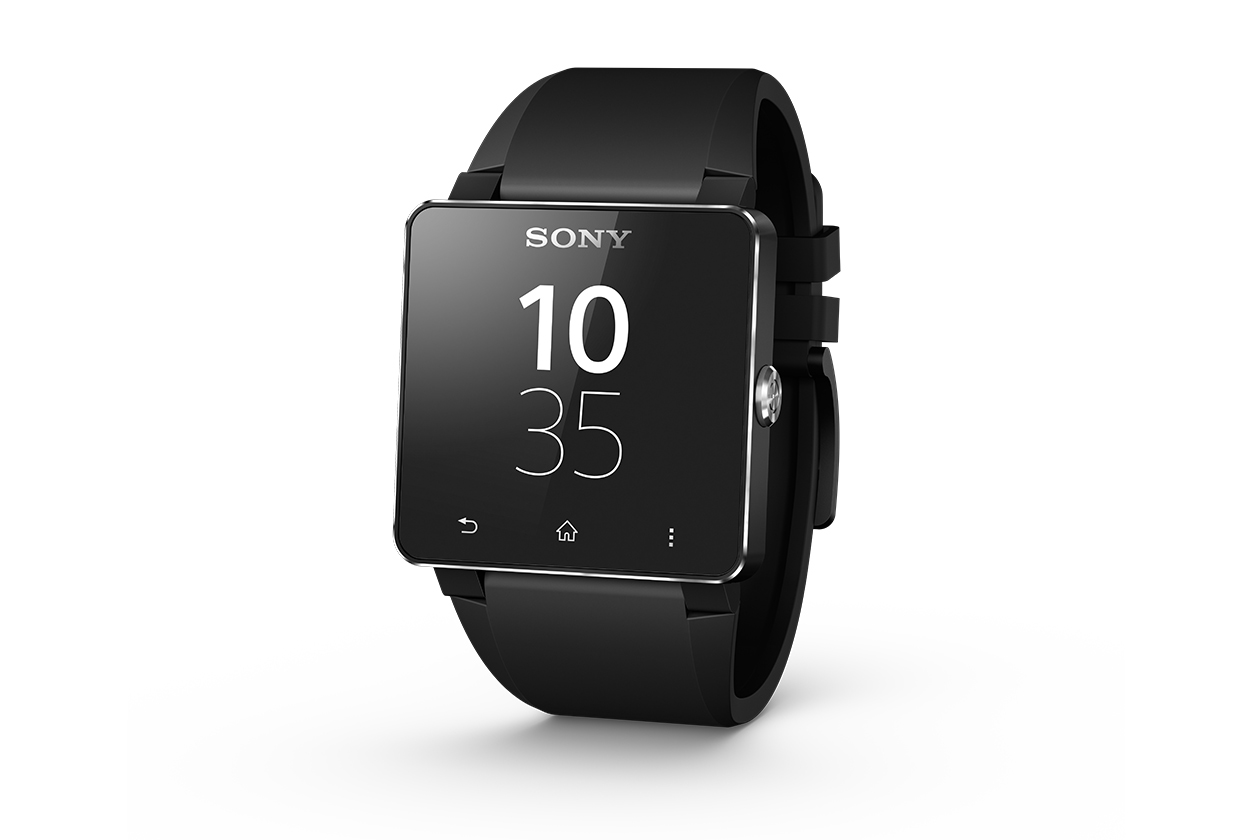
\includegraphics[width=200px]{images/sw2.jpg}
	\label{fig:sw2}
	\caption{Sony Smartwatch 2}
  \end{center}
\end{figure}
\newpage
All the Sony devices use an application called Smart Connect. This application keeps track of all the devices that want to make contact with the phone. It also keeps track of the applications that are installed on the watch. Whenever the pairing is stopped between the phone and the watch, all the previously installed applications are removed from the watch until these two devices are paired again.
\subsubsection{Smartwatch applications}
\label{subsubsec:sw_app}
%needs revision
The life cycle of a smartwatch app is about the same as an application on a phone or tablet. This can be seen in figure \ref{fig:sw2_lifecycle}. As stated before, the smartwatch apps only work when they are paired with the master device(the device which having the Smart Connect installed). When making an app, a few things are needed. First, register the app because it is needed for Smart Connect to find the app. \textbf{Register it to whom/where?}\pend
Then update the AndroidManifest.xml file that defines the programmer main activity and some control features. After this, the app can be coded by including the mandatory classes to make the application compatible with SW2. \pend  
Sony has made a level of abstraction that makes it easy to send messages using intents. As stated before, the pairing process is handled by the Smart Connect. 
\begin{figure}
\begin{center}
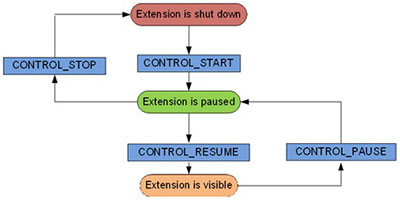
\includegraphics[scale=0.5]{images/applifecycle.jpg}
\end{center}
  \caption{Life cycle of a Sony smartwatch app}
  \label{fig:sw2_lifecycle}
  \captionsetup{font={footnotesize,bf,it}}
  \caption*{\url{https://developer.sony.com/develop/wearables/smartwatch-2-apis/guides/build-your-app/}}
\end{figure}